\documentclass[11pt]{scrartcl}

    \usepackage{ucs}
    \usepackage[utf8]{inputenc}
    \usepackage[T1]{fontenc}
    \usepackage[ngerman]{babel}
    \usepackage{amsmath,amssymb,amstext}
    \usepackage{graphicx}
    \usepackage{parskip}
    \usepackage{hyperref}
    \usepackage{float}
    \usepackage{subfiles}
    \usepackage{titling}
    \usepackage{ccicons}
    \usepackage{fontawesome}
    \usepackage{subfig}
    \usepackage[top=1in, bottom=1.25in, left=1.25in, right=1.25in]{geometry}
    \usepackage{xcolor}
    \usepackage{listings}
    \lstset{basicstyle=\small,
      showstringspaces=false,
      commentstyle=\color{black},
      keywordstyle=\color{blue}
    }

    \graphicspath{{images/}{../images/}}

        \title{Dokumentation - PREN}
        \author{A. Rebsamen, J. Grepper, M. Omlin, \\ M. Schöni, P. Marty, S. Ineichen}
        \date{\today{}, Luzern}

    \begin{document}

        \begin{titlingpage}
            \begin{center}
                \begin{Huge} %Exakter Modulnamen und Modulnamen ausgeschrieben
                    TA.BA{\_}PREN1.H1801 \\
                    \textbf{\thetitle} \\
                \end{Huge}
                \vspace{0.5cm}
                \begin{huge} %Author-Variable
                    \theauthor \\
                \end{huge}
                \vspace{0.5cm}
                \vspace{1cm}
                \begin{figure}[H] %Titelbild
                    \centering
                    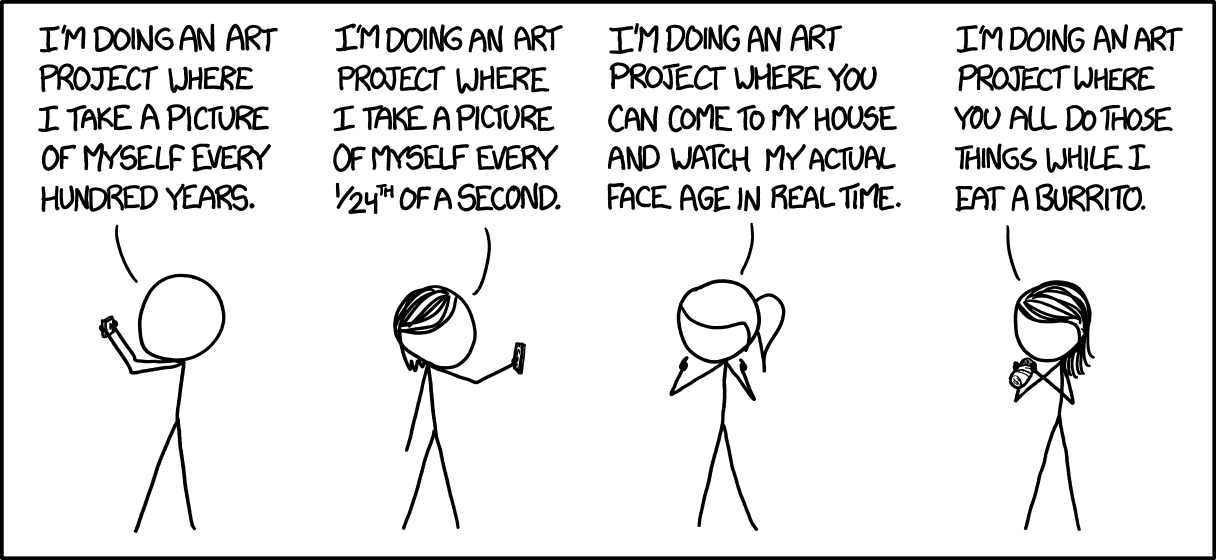
\includegraphics[width=0.6\textwidth]{images/comic.png}
                    \caption {https://xkcd.com/1496/}
                \end{figure}
                \vspace{0.5cm}
                \begin{huge} %Datumsvariable
                    \thedate
                \end{huge}
            \end{center}
        \end{titlingpage}

        %Inhaltsverzeichnis
        \tableofcontents
        \clearpage

        \section{Anforderungs Analyse}
        \subfile{sections/01_anforderungs_analyse/anforderungs_analyse.tex}
        \clearpage

        \section{Technologie Recherche}
        \subfile{sections/02_technologie_recherche/technologie_recherche.tex}
        \clearpage

        \section{Konzepte}
        \subfile{sections/03_konzepte/konzepte.tex}
        \clearpage

    \end{document}